\documentclass[useAMS, usenatbib, preprint, 12pt]{aastex}
\usepackage{cite, natbib}
\usepackage{float}
\usepackage{epsfig}
\usepackage{cases}
\usepackage[section]{placeins}
\usepackage{graphicx, subfigure}
\usepackage{color}
\usepackage{bm}

\bibliographystyle{aasjournal}

\newcommand{\Kepler}{{\it Kepler}}
\newcommand{\kepler}{\Kepler}
\newcommand{\corot}{{\it CoRoT}}
\newcommand{\Ktwo}{{\it K2}}
\newcommand{\ktwo}{\Ktwo}
\newcommand{\TESS}{{\it TESS}}
\newcommand{\LSST}{{\it LSST}}
\newcommand{\Wfirst}{{\it Wfirst}}
\newcommand{\SDSS}{{\it SDSS}}
\newcommand{\PLATO}{{\it PLATO}}
\newcommand{\Gaia}{{\it Gaia}}
\newcommand{\gaia}{{\it Gaia}}
\newcommand{\Teff}{$T_{\mathrm{eff}}$}
\newcommand{\teff}{$T_{\mathrm{eff}}$}
\newcommand{\FeH}{[Fe/H]}
\newcommand{\feh}{[Fe/H]}
\newcommand{\ie}{{\it i.e.}}
\newcommand{\eg}{{\it e.g.}}
\newcommand{\logg}{log \emph{g}}
\newcommand{\dnu}{$\Delta \nu$}
\newcommand{\numax}{$\nu_{\mathrm{max}}$}

\newcommand{\racomment}[1]{{\color{red}#1}}

\newcommand{\columbia}{1}
\newcommand{\simons}{2}
\newcommand{\ww}{3}
\newcommand{\nsf}{4}
\newcommand{\florida}{5}
\newcommand{\cca}{6}
\newcommand{\hubble}{7}
\newcommand{\princeton}{8}

\begin{document}

\title{Investigating magnetic dynamo evolution with TESS field dwarfs}

\author{R. Angus\altaffilmark{\columbia}
% \altaffilmark{\simons}
        J. R. Davenport\altaffilmark{\ww}
% \altaffilmark{\nsf},
        D. Busazi\altaffilmark{\florida},
        D. Foreman-Mackey\altaffilmark{\cca},
        A. Mann\altaffilmark{\columbia}
% \altaffilmark{\hubble},
        S. Oh\altaffilmark{\princeton},
        D. Kipping\altaffilmark{\columbia}
}

\altaffiltext{\columbia}{Department of Astronomy, Columbia University, New
York, NY}
\altaffiltext{\simons}{Simons Fellow, RuthAngus@gmail.com}
\altaffiltext{\ww}{Western Washington University, Bellingham, WA}
\altaffiltext{\nsf}{NSF Fellow}
\altaffiltext{\florida}{Florida Gulf Coast University, Fort Myers, FL}
\altaffiltext{\cca}{Center for Computational Astronomy, Flatiron Institute,
New York, NY}
\altaffiltext{\hubble}{Hubble Fellow}
\altaffiltext{\princeton}{Princeton University, Princeton, NJ}

\section{Introduction}

Galactic archaeology and exoplanet populations are two rapidly accelerating
fields of interest within astronomy.
Although seemingly unconnected, these fields are linked by a mutual
requirement for precise stellar parameters.
To galactic archaeologists, ages and elemental abundances are the most
important parameters.
Indeed, most galactic archaeology surveys target exactly these properties.
For exoplaneteers, masses and radii have historically been the most important
stellar parameters for understanding planetary systems.
With a growing number of planet hosts with precise masses and radii, attention
is turning toward other parameters, such as ages, to understand the history
and evolution of these systems.
Age is therefore a fundamental stellar parameter of great interest to at least
two large communities of astronomers.
Unfortunately however, it is a difficult attribute to measure for main sequence
F, G, K, and M stars in the field, in part because low-mass dwarfs do not move
far on the Color-Magnitude diagram (CMD) during their hydrogen burning
lifetimes.
Further, competing stellar evolution models predict different ages for the
same star.
Of the measurable properties for a large ensemble of field stars, rotation
periods contain the most information about stellar age, and provide the best
leverage for advancing our knowledge of galactic archeology as well as
exoplanet population demographics via gyrochronology.

Angular momentum is carried away though magnetically driven stellar winds,
which slows the star’s rotation over cosmic time.
This rotation-based `clock' is known as gyrochronology.
Cool spots on the star’s surface rotate in-to and out-of view, creating small
amplitude ($\pm$ 1\%) quasi-periodic changes in the stellar brightness.
While rotation periods have previously been measured from starspot-induced
flux modulations for hundreds of stars from the ground, space-based
photometric surveys have opened the door to homogeneous ensemble measures of
stellar rotation, and therefore age.
Using precise light curves available from the TESS mission, we hope to
infer ages for nearly 100,000 main sequence field stars, including thousands
of planet hosts.
The ages of the planet hosts will allow us to characterize trends in planet
properties over time.

Additionally, as rotation both influences and is influenced {\it by} stellar
magnetic fields, it is inextricably related to stellar activity.
With so many TESS targets being M dwarfs which tend to be particularly active,
understanding the magnetic behavior of these stars has never been more
important.

To enable studies of stellar ages and magnetic activity from rotation periods
with TESS, we propose to:
1. Measure accurate rotation periods for every available TESS FFI and
two-minute cadence target.
2. Produce updated gyrochronology relations based on a wider range of field
star ages.
3. Determine the origin of the mysterious rotation period bimodality
discovered with Kepler by tracing the rotation period distribution over the
whole sky, and out to further distances utilizing public Gaia data.
4. Measure the star formation history across the sky using a new Bayesian
age-dating system.
5. Further characterize the intrinsic uncertainty in gyrochronology ages using
comoving pairs identified in the first Gaia data release.

\section{Scientific Justification}
\subsection{Rotation period bimodality}

One of the most remarkable results from the Kepler rotation period catalog was
the discovery of a bimodal period distribution among field stars by
\citet{mcquillan2013}, which is shown in Figure \ref{fig:davenport}.
While a separate sequence of rapid rotation periods had been known in young
stellar clusters due to lower-mass stars settling on to the angular momentum
main sequence slower \citep[\eg][]{barnes2007}, this new bimodality was
detected from slower rotating M dwarfs (T$_\mathrm{eff} <$ 4000).
The bimodality separated M dwarfs into two populations, those with rotation
periods longer than $\sim$ 20 days, and those with periods between $\sim$ 1
and 20 days.
Follow-up analysis of the Kepler data by \citet{mcquillan2014} found the
period bimodality extended to include K dwarfs.
Recently, Co-I Davenport discovered this period bimodality extends throughout
all masses in the Kepler rotation sample for nearby stars, as shown in Figure
\ref{fig:davenport} \citep{davenport2017}.
Two formation scenarios have been proposed to explain the observed period
bimodality.
The first scenario, initially proposed by \citet{mcquillan2013}, is the
rotation period distribution reflects the local star formation history, and
thus the bimodality represents a drop in the star formation rate around 600
Myr ago.
This model is supported by both the extension of the bimodality to earlier
spectral types by \citet{davenport2017}, and also the tentative detection that
the two rotation period populations have distinct proper motion distributions.
However, such a variation in the star formation rate on short timescales has
some tension with independent observational efforts to determine the local
star formation history.
While Color–Magnitude diagram inversions from Hipparcos have suggested a
similarly short timescale variation in star formation of $\sim$ 0.5 Gyr
\citep{hernandez2000}, other studies find slower variations over several
Gyr \citep[\eg][]{cignoni2006}.
Using white dwarf cooling models to infer the local formation history
(“cosmochronology”) also supports higher star formation several Gyr ago, but
can rarely achieve age resolution better than $\sim$ 1 Gyr due to small sample
sizes \citep{tremblay2014}.
The spatial extent of such coherent and localized variations in star formation
history is unknown.
The second scenario to explain this feature is that the period bimodality
occurs due to a previously unknown variation in the spin-down evolution for
low-mass stars.
In this model the star formation history would be continuous over the past
$\sim$ 1 Gyr, and around 600 Myr stars would move quickly through the observed
period minima due to this unknown phase transition or feedback mechanism.
While this model is not predicted by angular momentum loss prescriptions,
rapid transitions in rotation period are observed for stars in young clusters.
Stars move quickly from the rapidly rotating “convective” sequence (periods of
$\sim<1$ day) to the “interface” sequence (periods of several days) during the
first few hundred Myr, with lower mass stars taking longer to make this
transition as they settle onto the main sequence \citep{barnes2003}.
Secondly, a gap in chromospheric activity levels for solar-type field stars
has also been observed \citep{vaughan1980}.
While this magnetic activity indicator smoothly varies with stellar ages over
long timescales, the gap indicates a rapid transition phase from “active” to
“inactive” is present within the first Gyr \citep{pace2009}.
Thirdly, the angular momentum loss underpinning gyrochronology seems to slow
for stars older than the Sun, indicating a potential change in the magnetic
dynamo for slower rotators \citep{angus2015, van-saders2016}.

The TESS FFI and CTL targets will provide the ideal dataset to test these two
formation scenarios.
If the bimodality is due to an age distribution we would expect only to see
the feature locally; it could disappear at greater distances or along
different lines of sight where small scale variations in the star formation
history are less apparent.
However, if the bimodality is truly due to a transition point in the spin-down
evolution at young ages, we would expect to find no little to no variation in
this feature as seen in Figure \ref{fig:davenport} with galactic position.

To map the rotation period distribution as a function of galactocentric
position we will match the TESS FFI and CTL targets to the upcoming data
release from the Gaia mission \citep{perryman2001}.
This will also allow us to remove contaminating subgiants and binary stars
from the sample, leaving only single main sequence stars.
The period distribution of G dwarfs is critical for this analysis since they
are observable at greater distances, allowing us to sample different star
formation histories.
With the April 2018 data release from Gaia (DR2) estimate that we will be able
to study rotation periods for G dwarfs in the TESS FFIs out to $\sim$ 3 kpc.
Unlike \Kepler, since \TESS\ is targeting the whole sky, it will be possible
to investigate the rotation period distribution as a function of
galactocentric position.
The size scale over which the Milky Way’s star formation history varies is
unknown however significant variations in star formation histories are seen in
Andromeda between 100 pc volumes, as well as large galaxy-wide trends
\citep[\eg][]{lewis2015}.

\begin{figure}
\begin{center}
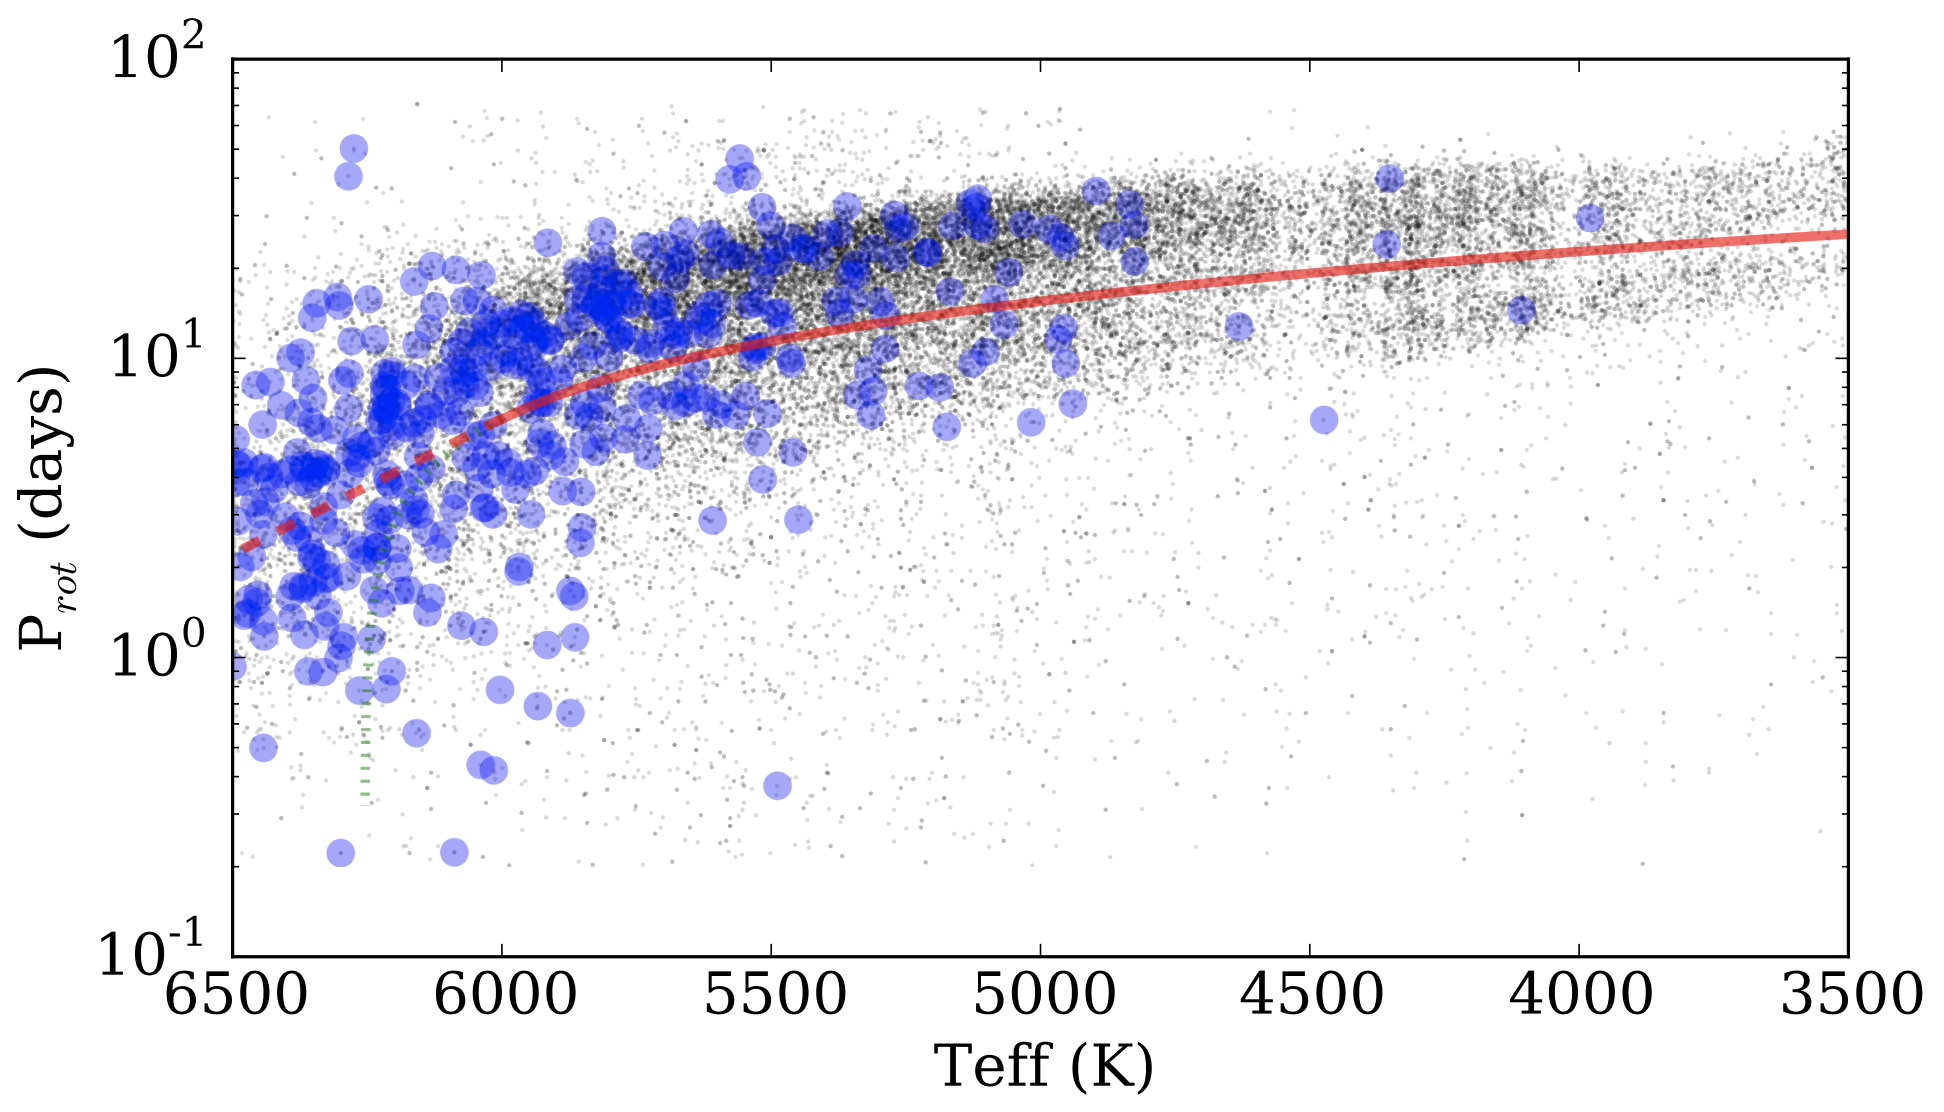
\includegraphics[width=3in, clip=true]{Davenport.png}
\caption{From Davenport (2017).
    Rotation period as a function of effective
temperature for the full McQuillan et al., (2014) Kepler sample in black, and
the subset of these stars that also feature in the TGAS Gaia DR1 catalogue in
blue. Contaminating giants have been removed from the blue sample and the
rotation period bimodality is revealed to exist across all temperatures shown.
    The red line is a 600 Myr rotational isochrone (also known as a gyrochrone).}
\label{fig:davenport}
\end{center}
\end{figure}

\subsection{Gyrochronology}

Gyrochronology is by far the most widely applicable, relatively precise
age-dating method available.
Although the phenomenon of magnetic braking has been closely studied since its
discovery in the mid/late 20th century, the manifestations of magnetic fields
and their effects on rotation and activity are complex; the physics
underpinning rotational evolution are far from well-understood.
Although the classical spin-down law of \citet{skumanich1972}: Period
$\propto$ Age$^1/2$ holds for all open clusters with measured periods, it does
not appear to describe old field stars \citep{angus2015, van-saders2016}.
Asteroseismic pulsators observed by Kepler, older than the Sun, rotate more
rapidly than the \citet{skumanich1972} law predicts they should.
\citet{van-saders2016} find that including a transition to a weakened magnetic
braking regime in the gyrochronology models, at a critical Rossby number,
provides an improved fit to the data.
Once a star reaches a critical Rossby number (the ratio of the rotation period
to the convective overturn time), magnetic braking efficiency effectively
drops to zero.
This means a 5 Gyr star of Solar mass will have the same rotation period as a
6 Gyr and rotation period cannot be used as an age proxy.
The transition occurs at around Solar age for Solar mass stars but later for
less massive stars and earlier for more massive stars.
Although this effect reduces the usefulness of gyrochronology for stars more
massive than the Sun, in practise, for Solar-mass stars, down to M dwarfs with
masses greater than 0.35$M_\odot$, gyrochronology can still be considered an
effective dating method.
This will include a large number of \TESS\ planet candidates.

We intend to use the rotation periods of planet hosting stars to infer the
age-dependence of planet frequency.
Kepler alone has not yet produced a sufficient number of stars with rotation
periods to reliably characterise the time-dependent frequency of exoplanets.
Mann et al. (2016a), Mann et al. (2016b) and Rizzuto et al. (2017) detected
transiting exoplanets in four young open clusters observed by the K2 mission.

\section{Measuring Rotation Periods}
In this era of large photometric surveys (Kepler/K2, TESS, WFIRST, LSST, PTF,
PanStarrs and more) rotation periods are quickly becoming one of the most
accessible properties of stars.
Precise light curves produced by these surveys often reveal the presence of
dark spots on the surfaces of cool stars which revolve with the stellar
surface creating an overall dimming effect once every rotation period.
Dark spotted regions and bright faculae leave a characteristic trace in the
light curve from which a rotation period can be inferred.
The extraction of a rotation period from a light curve can be as
straight-forward as computing a Lomb-Scargle periodogram or, in cases where
the signal is less clear, can be inferred via modelling the correlation
between data points.
This latter approach could involve either computing an autocorrelation
function (McQuillan et al., 2013), or fitting a Gaussian process to the time
series (Angus et al., 2017, Foreman-Mackey et al., 2017).
Signals produced by the rotation of spotted stars can have amplitudes of a few
percent of the total flux, but can also have very low amplitudes of a few
parts per million.
The frequencies of high amplitude signals are easy to measure and, in these
cases, most measured frequencies will agree regardless of the technique used
to measure them.
Similarly, short-period signals are easy to measure, especially if light curve
variations are sinusoidal in shape.
In the low amplitude and long period cases however, care is needed to separate
real astrophysical signal from instrumental systematics.

The measurement of rotation periods is less sensitive to crowding and source
confusion than exoplanet transit characterization because the rotation period
is not effected by photometric dilution.
We will apply two complementary methods to extract and calibrate light curves
from the TESS FFIs.
First, for bright or isolated targets, we will follow \citet{montet2017} to
estimate aperture shapes and perform aperture photometry for bright sources.
Using an ensemble of sources, we will de-trend these light curves using a
modified version of \textsf{everest} \citep{luger2016, luger2017} designed to
preserve photometric signatures of rotation.
This will be achieved by fitting for the systematic effects in the light curve
using the \textsf{everest} model simultaneously with a Gaussian Process model
for the astrophysical variation.
Both \citet{aigrain2016} and \citet{luger2016} demonstrated that this can
preserve stellar variability signals and we will use the \textsf{celerite}
algorithm \citep{dfm2017} to scale the computations to the size of TESS FFI
datasets.

The precision of existing photometric de-trending methods degrades in crowded
fields \citep[for example,][]{luger2017}.
However, to make robust measurements of rotation periods, we do not need
absolutely calibrated light curves.
Therefore, in crowded fields, we will apply a difference imaging method that
was developed for the K2 Campaign 9 microlensing project \citep{henderson2016}
based on the \textsf{CPM} \citep{wang2016} to robustly measure the photometric
variations of crowded sources.
Unlike standard difference imaging methods, this procedure does not require a
reference image.
Instead, a causal data-driven model is built to predict the time series in
every pixel taking systematic effects into account and the residuals between
the observations and the model predictions provide an estimate of the
astrophysical variability in each pixel.
We will tune this method preserve rotation signals and apply it to detect
rotation across the FFIs.


\begin{figure}
\begin{center}
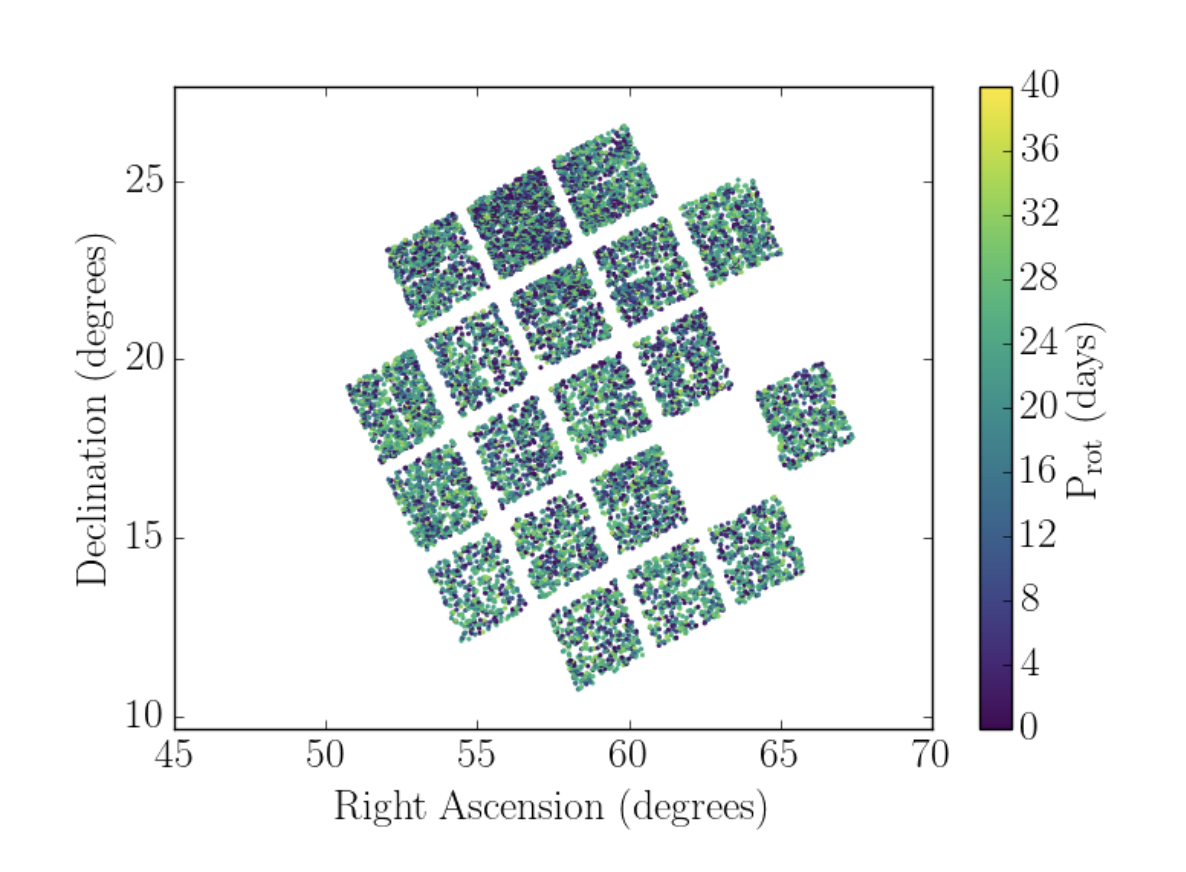
\includegraphics[width=6in, clip=true]{Kalesalad.png}
\caption{All stars observed during K2 campaign 4, plotted according to their
equatorial coordinates and colored by their preliminary rotation period.
These rotation periods were measured using a simple ACF method, applied to
    everest (Luger et al., 2015) light curves.}
\label{fig:kalesalad}
\end{center}
\end{figure}

We intend to measure rotation periods for all mid to low-mass dwarfs that show
evidence of rotational modulation in their light curves.

Need to measure rotation periods of all stars if you want to infer the
distribution of planets as a function of age.

It looks like hotter stars stop spinning down at around the age of the Sun.
However, that does not necessarily mean that gyrochronology cannot be used to
infer ages.
Gyro works for low mass stars down to around 0.35 M$_\odot$ (CITATION), up to
the age of the Universe.
It works for Solar-mass stars up to the age of the Sun and for stars more
massive than the Sun (but less massive than the Kraft break) it works to
gradually decreasing ages.
This means that X\% of stars in the TIC are likely to have ages that can be
determined by gyrochronology.

\section{Expected Impact}
We will provide light curves and rotation periods for both the two-minute
cadence and FFI targets.

\section{Budget Justification}
PI Angus intends to use the budget to employ a student for 3-4 months.
In this time the student will assist in extracting light curves from the FFIs,
measuring rotation periods and building a rotation period catalog.
The student will also be involved in the scientific project of their choosing:
either the rotation period bimodality, gyrochronology of low-mass stars, or
gyrochronology of comoving pairs.

\bibliography{references}

\end{document}
